%%%%%%%%%%%%%%%%%%%%%%%%%%%%%%%%%%%%%%%%
%%%%% RESULTS
%%%%%%%%%%%%%%%%%%%%%%%%%%%%%%%%%%%%%%%%
\section{RESULTS}
	In this section, we discuss the results for each model type: single layer and two layer LSTM, the model that performed best 'universally' across almost every user, the best performing model per user, and the best performing models for a single user (User 3). User 3 was chosen not because they had the best performance out of all users, as User 2 had that distinction, but rather User 3 has a balance of significant improvement and performance. An examination of poor performance is also included as to be transparent and address criticisms of our approach. 
    It is worth noting that for all of the following figures and discussions, the metric for the loss is the mean squared error (MSE) of the standardized play counts. In other words, an MSE of 1 means that the error by the network was $\pm1$ standard deviation. Over all experiments, user 1 had the worst performance, with no final MSE being under 1 standard deviation.
    
%%%%%%%%%%%%%%%%%%%%%%%%%%%%%%%%%%%%%%%%
%%%%% 1 LAYER
%%%%%%%%%%%%%%%%%%%%%%%%%%%%%%%%%%%%%%%%
	\subsection{Single Layer Model Results}
    Depicted in figure \ref{fig:results-1-layer} is the single layer LSTM model that had the best improvement for each user. These models are not necessarily the ones with the best performance overall. As can be seen, the number of time steps varied greatly, however in the majority of cases, the best improvements came from models with $\geq 10$ time steps. In this case, excluding User 1, the MSE for each model was $<1$ standard deviation.
        \begin{figure}
            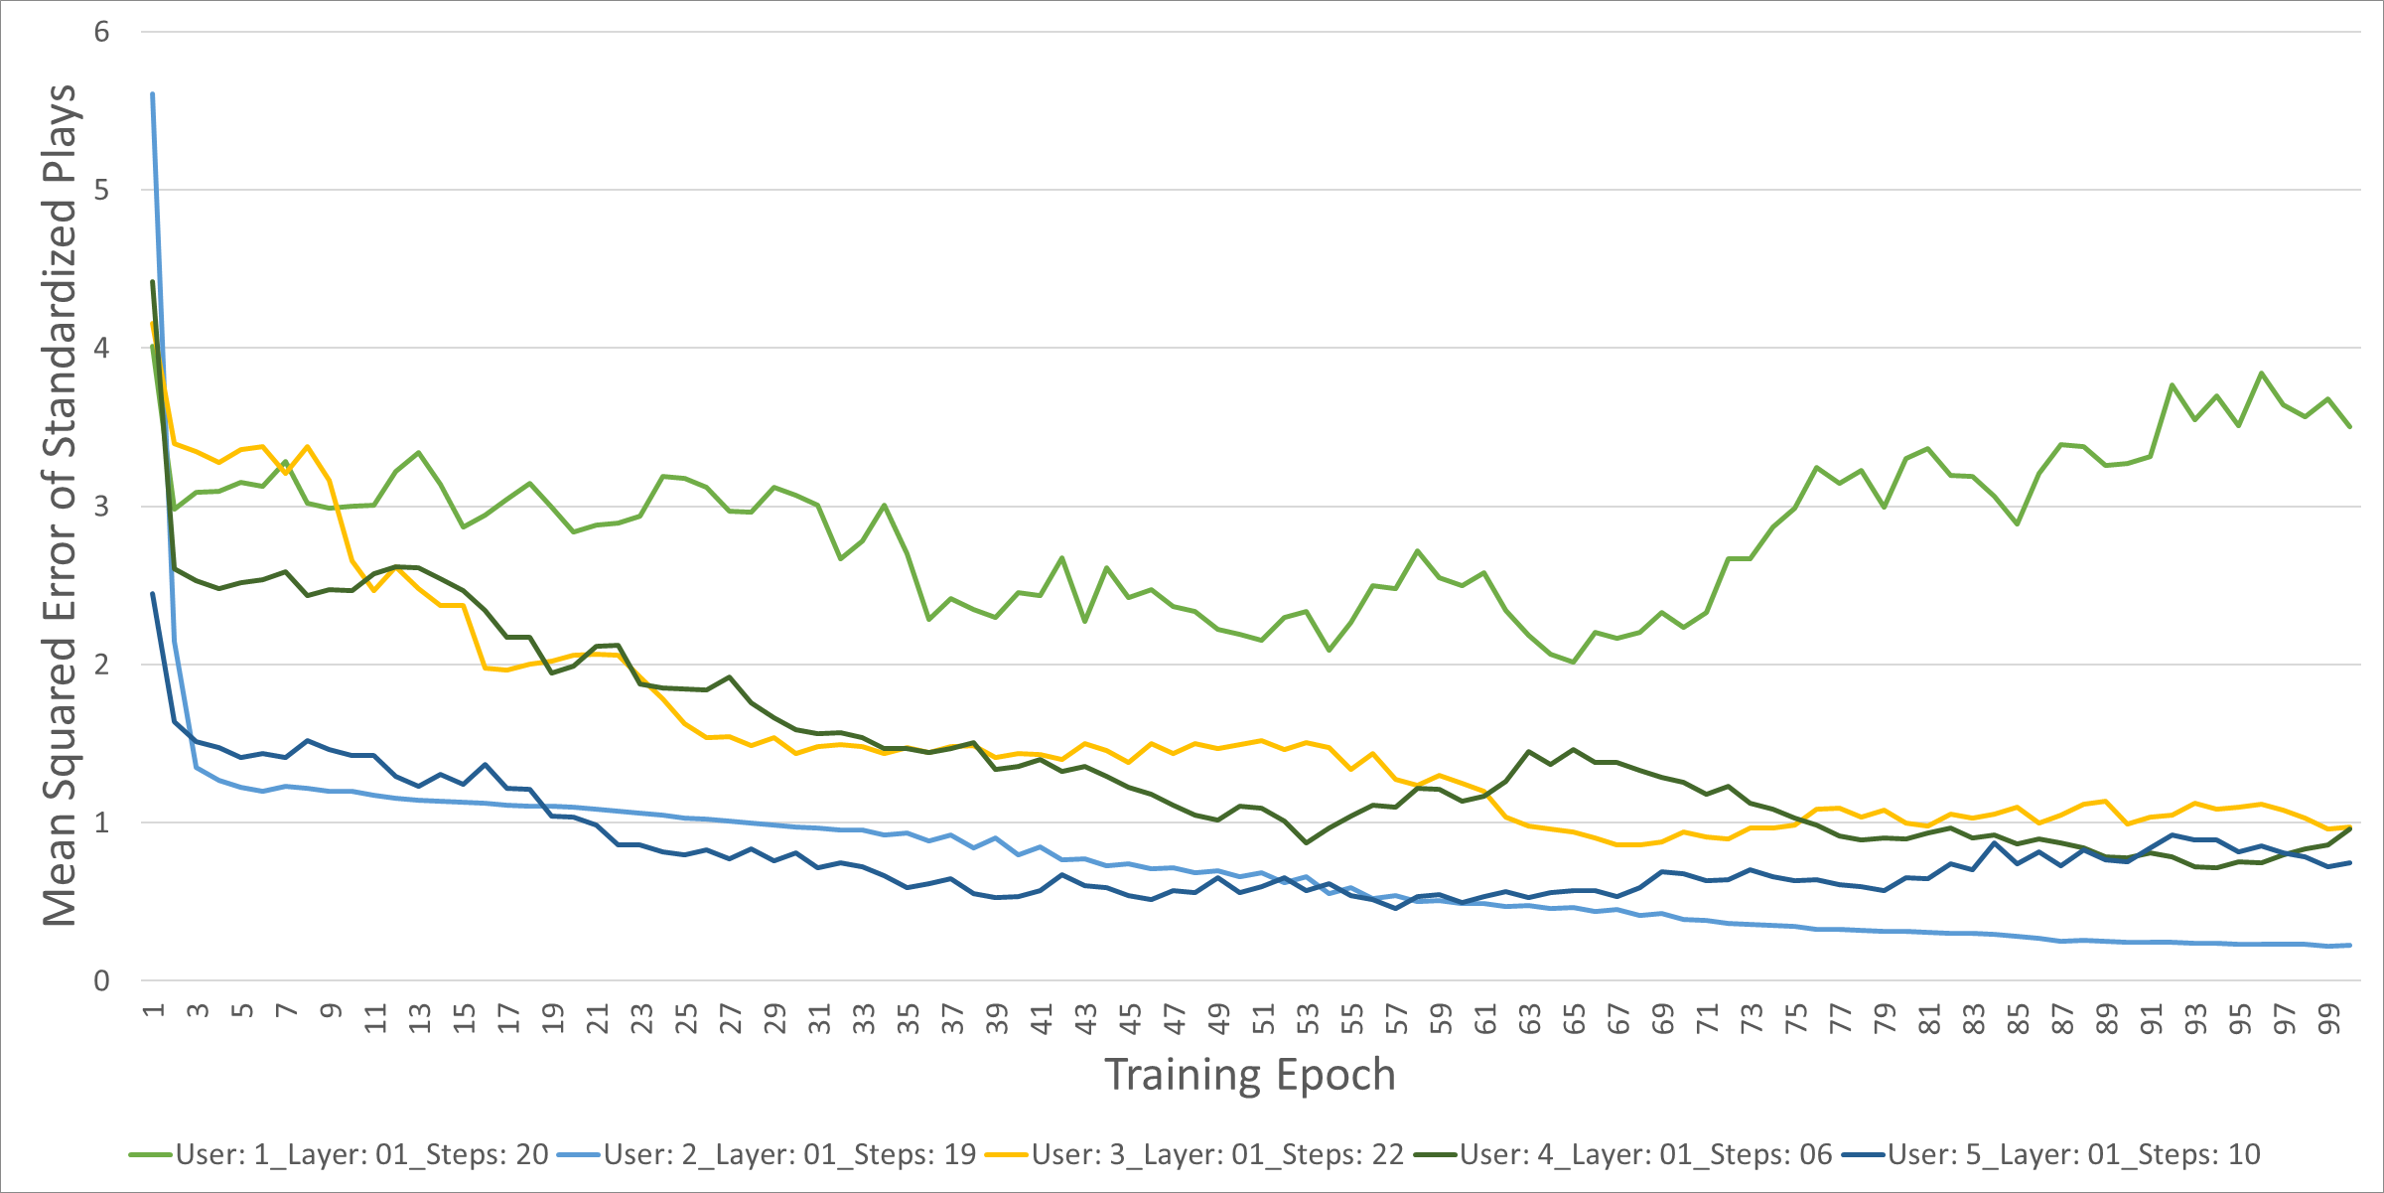
\includegraphics[width=0.45\textwidth]{result_best_1_layer.png}
            \caption{Best Performing Single LSTM Layer Model Per User}
            \label{fig:results-1-layer}
        \end{figure}
        
%%%%%%%%%%%%%%%%%%%%%%%%%%%%%%%%%%%%%%%%
%%%%% 2 LAYERS
%%%%%%%%%%%%%%%%%%%%%%%%%%%%%%%%%%%%%%%%
    \subsection{Two Layer Model Results}
    Similar to the prior subsection, figure \ref{fig:results-2-layer} displays the two layer models with the most improvement per user. As can be seen, in most cases the performance of the two layer LSTM models is significantly better than the single layer models. Excluding User 1, all of these models use $\geq 16$ time steps, further indicating that a longer time history improves the performance of the network.
        \begin{figure}
            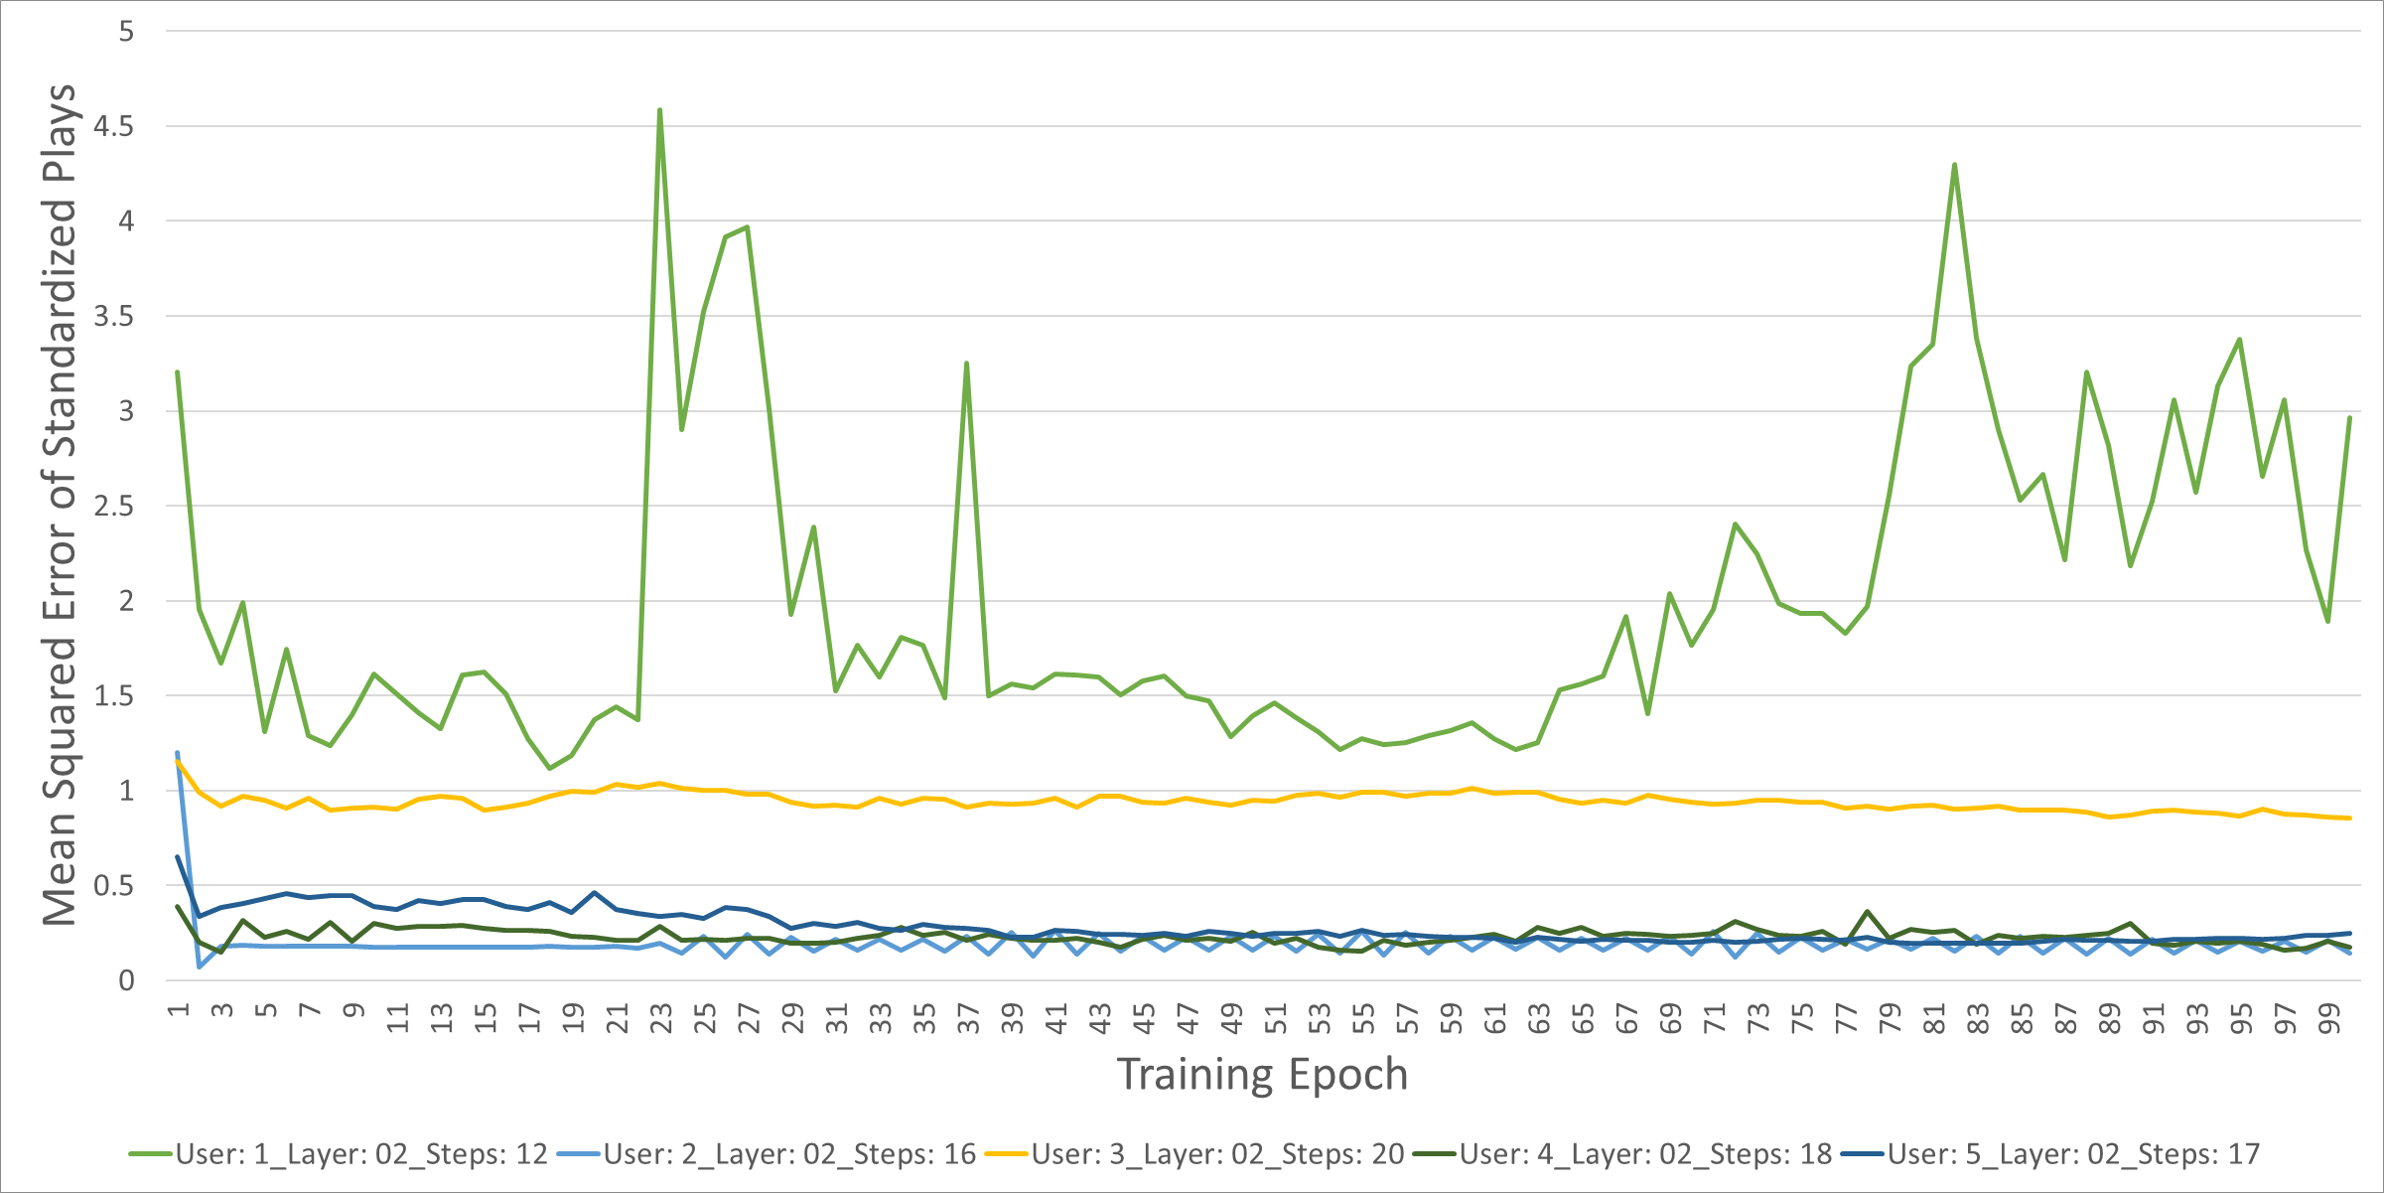
\includegraphics[width=0.45\textwidth]{result_best_2_layer.png}
            \caption{Best Performing Two LSTM Layer Model Per User}
            \label{fig:results-2-layer}
        \end{figure}
        
%%%%%%%%%%%%%%%%%%%%%%%%%%%%%%%%%%%%%%%%
%%%%% UNIVERSAL
%%%%%%%%%%%%%%%%%%%%%%%%%%%%%%%%%%%%%%%%  
    \subsection{Universal Model}
    While no model performed best for every single user, the combination of two LSTM layers and 18 time steps was the closest model to achieving that goal and the performance of this model is plotted in figure \ref{fig:results-overall}. In this case User 1's performance was divergent, however all other users had a final MSE of $<1$ and User 2-4 had a final MSE $<0.4$ standard deviations. Once again, this supports the assumption that a larger history for the LSTM to consider provides better performance.
        \begin{figure}
            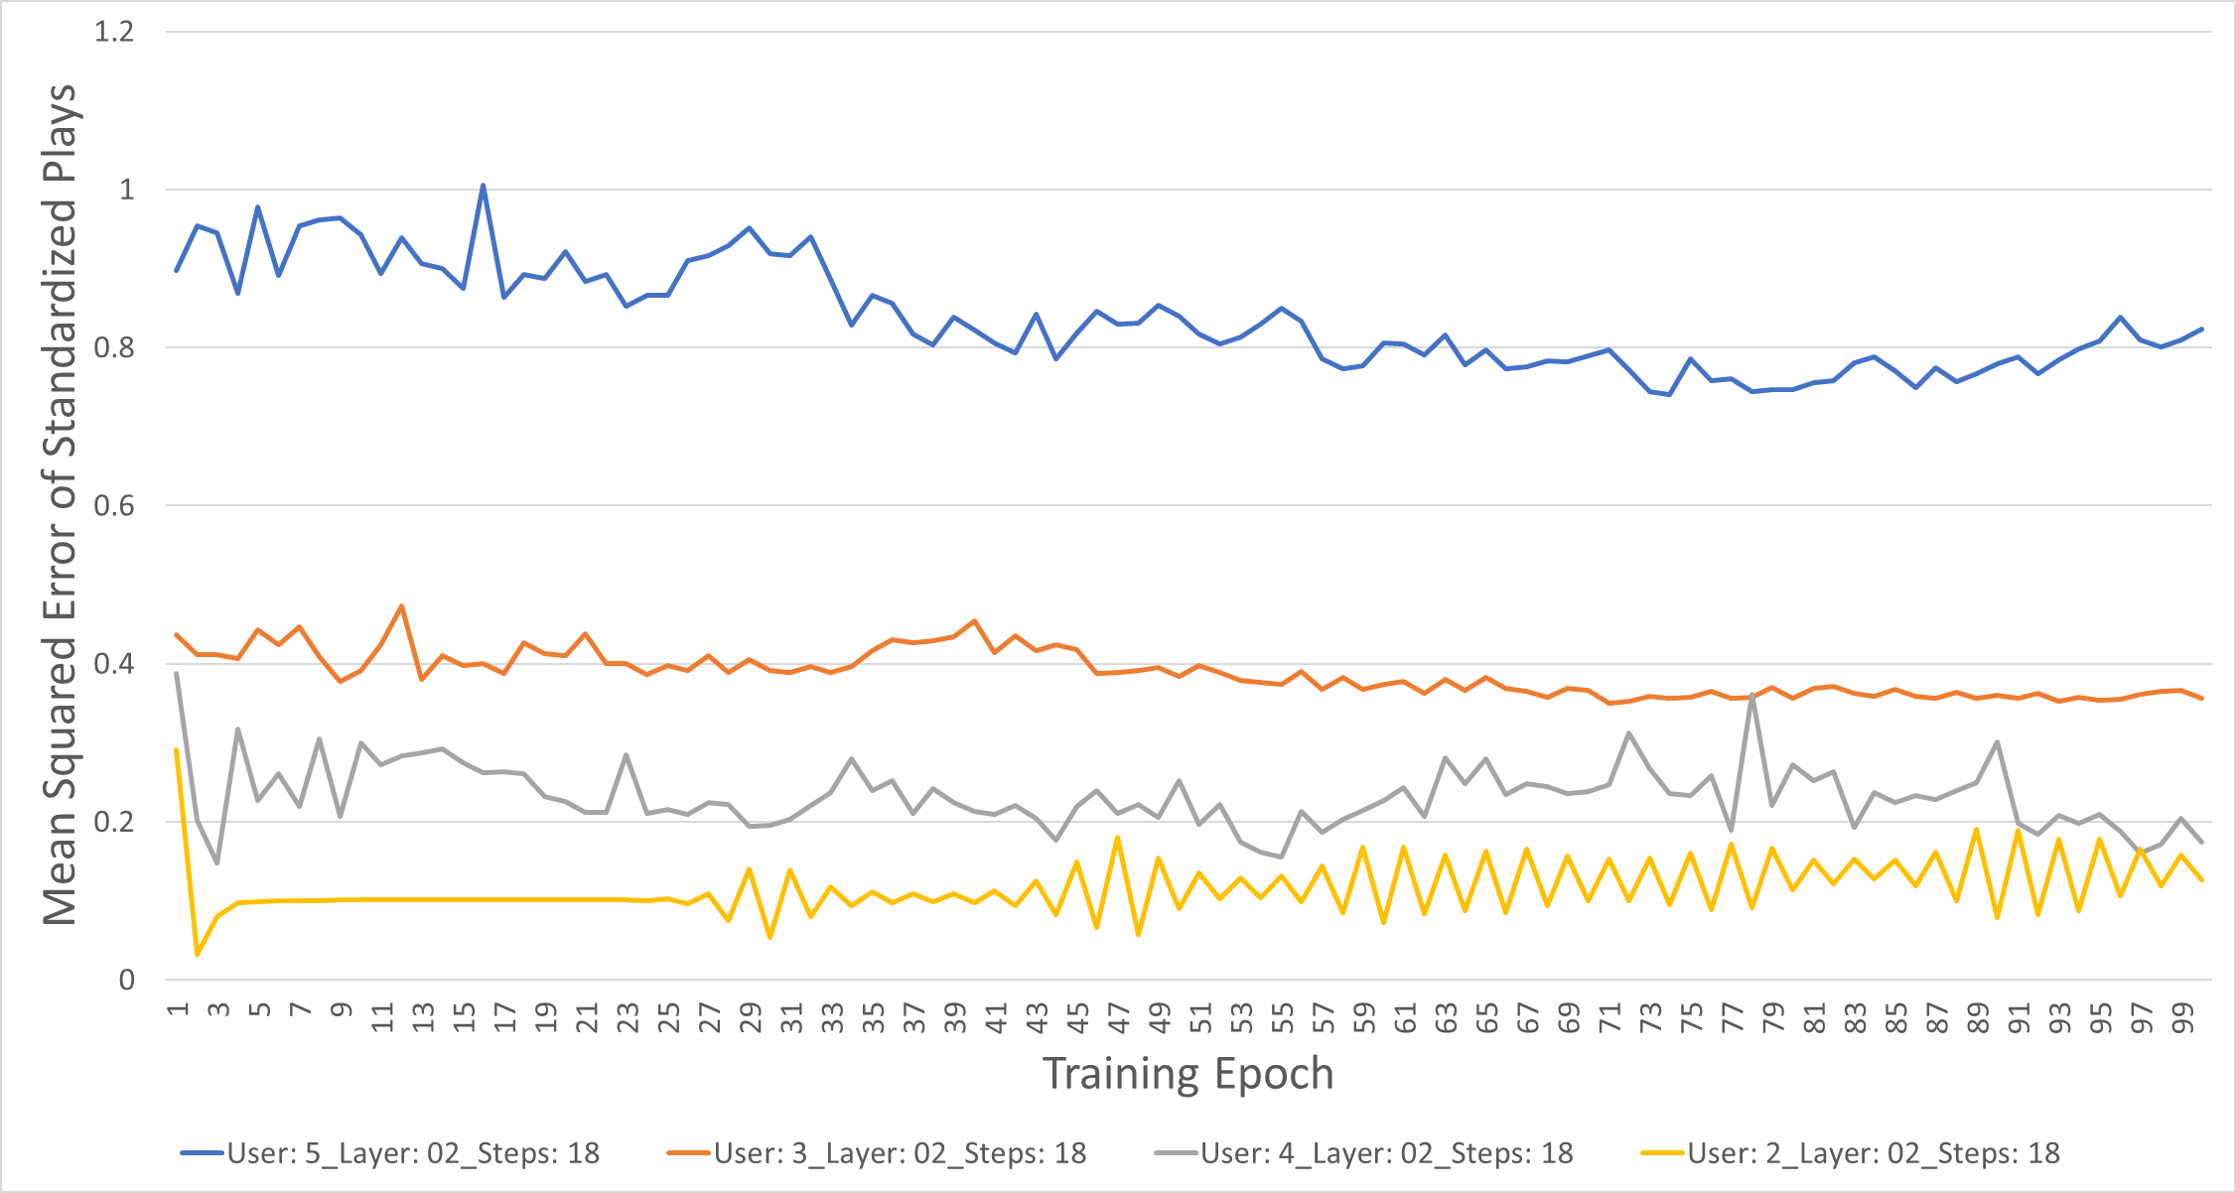
\includegraphics[width=0.45\textwidth]{result_best_overall.png}
            \caption{Best Universally Performing Model: 2 Layers 18 Time Steps}
            \label{fig:results-overall}
        \end{figure}
      
%%%%%%%%%%%%%%%%%%%%%%%%%%%%%%%%%%%%%%%%
%%%%% BEST PER USER
%%%%%%%%%%%%%%%%%%%%%%%%%%%%%%%%%%%%%%%%
    \subsection{Best Model Per User}
    Next we examine the best models in terms of performance per user and a sample of models for User 3 demonstrating excellent improvement and overall performance. Firstly, in figure \ref{fig:results-best-per-user}, for Users 2-5, the final performance was MSE $<0.4$, which is better than a random guess at the standardized number of plays for that user. User 5 had the best performance of all users, with the best performing model having a MSE $<0.06$.
        \begin{figure}
            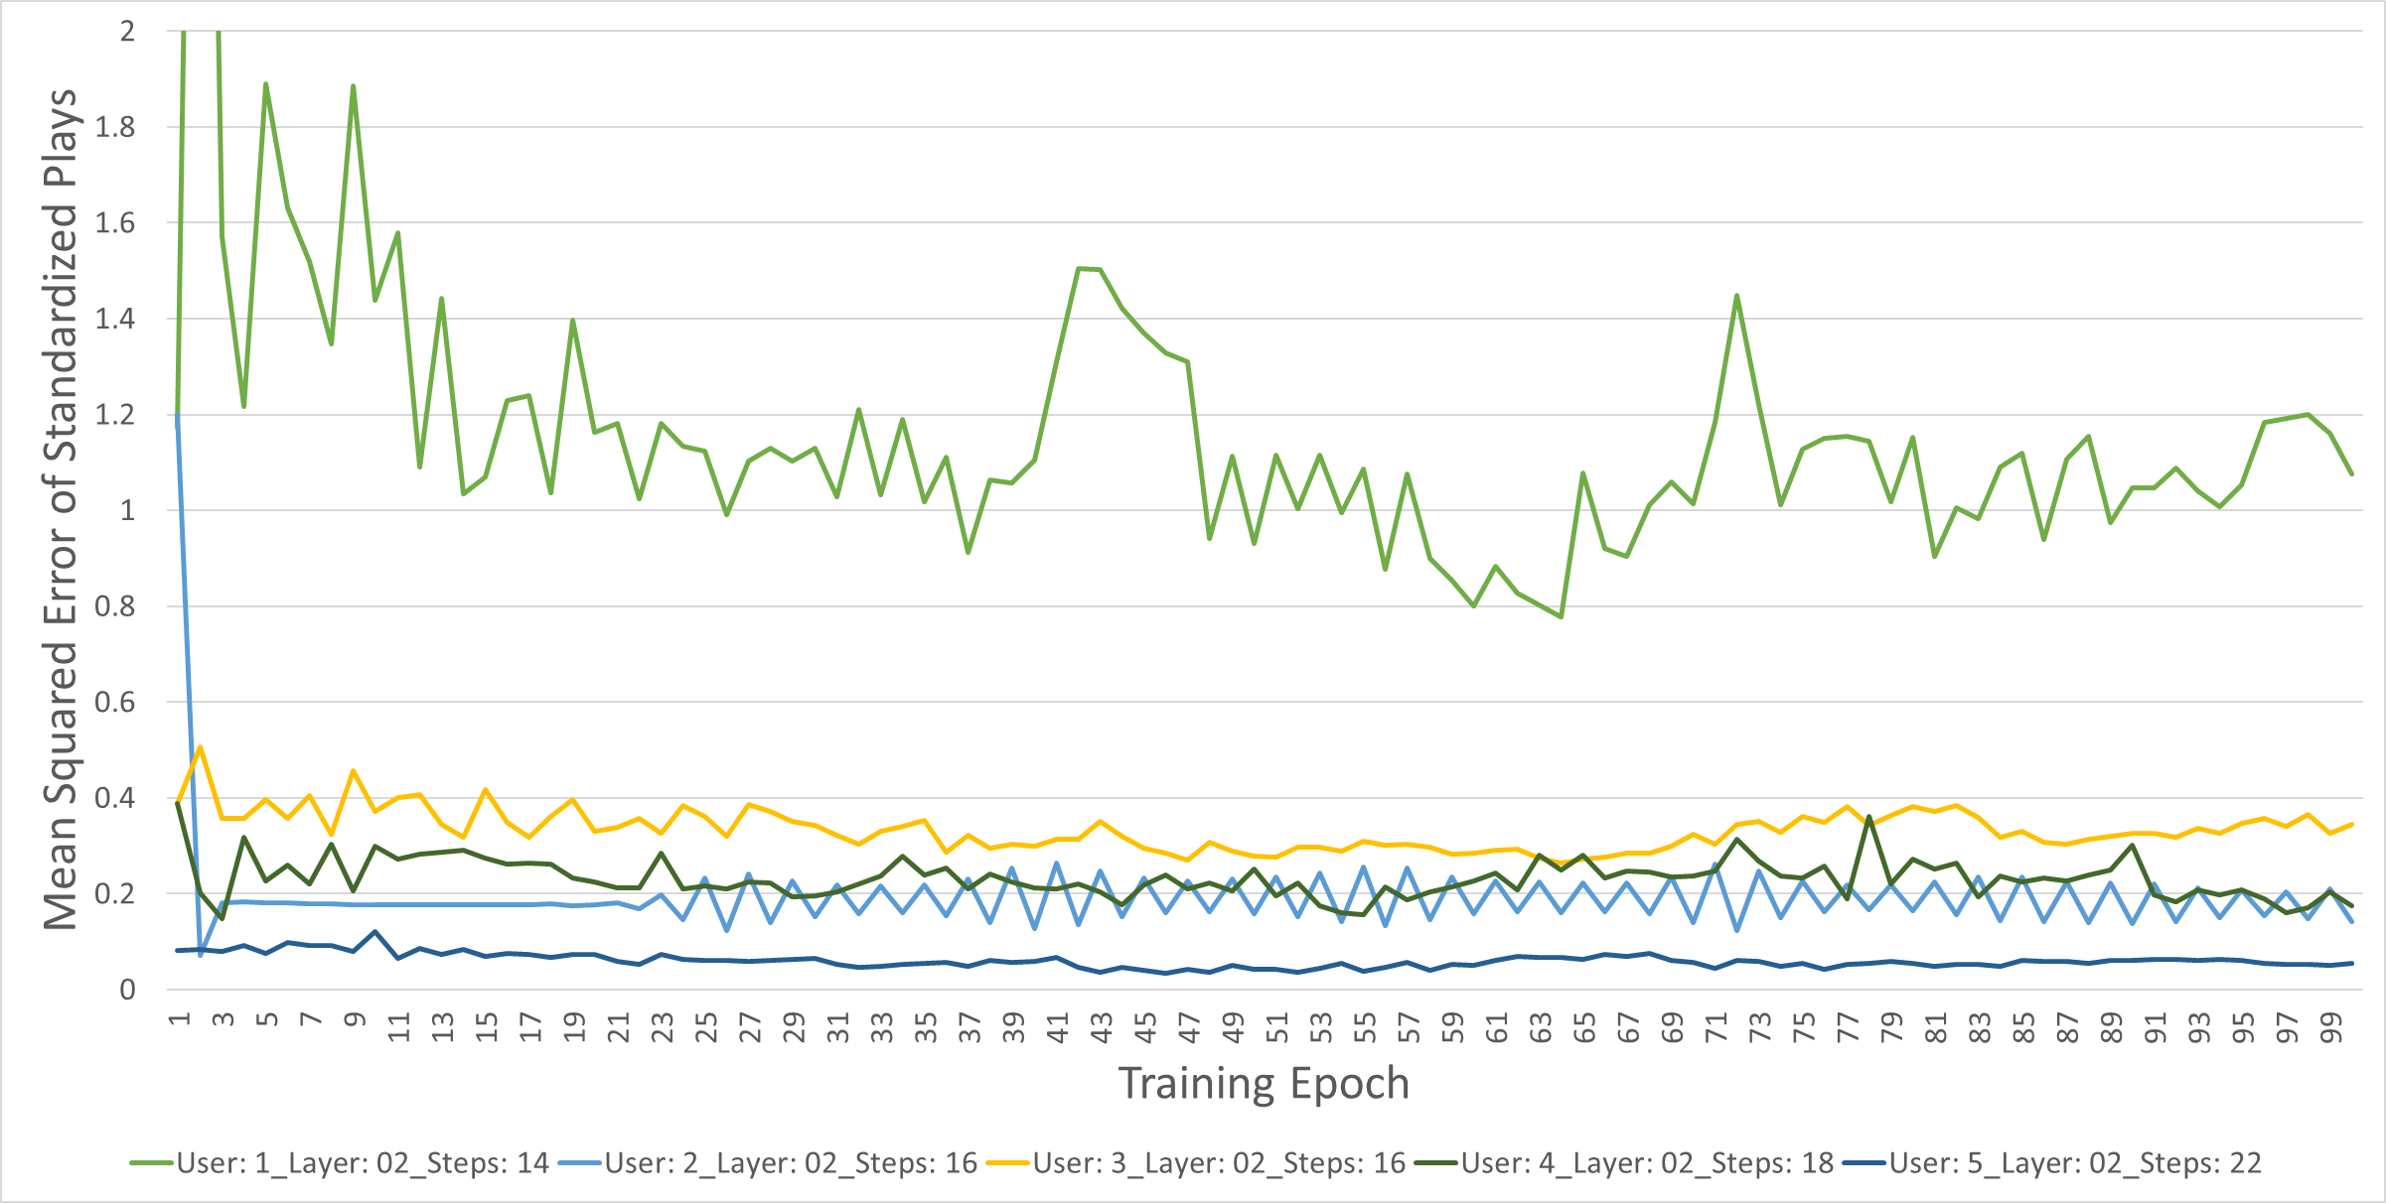
\includegraphics[width=0.45\textwidth]{result_best_per_user.png}
            \caption{Best Performing Model Per User}
            \label{fig:results-best-per-user}
        \end{figure}
        
    In figure \ref{fig:results-user-3}, multiple combinations of models are displayed over all 100 training epochs. In this case, the best performing models were under 0.5 MSE, however all models converged to an MSE of $<1$ standard deviation. The combination of 1 LSTM layer and 22 Time Steps is particularly impressive, converging to $<1$ MSE from $>4.15$ MSE at the first iteration.
        \begin{figure}
            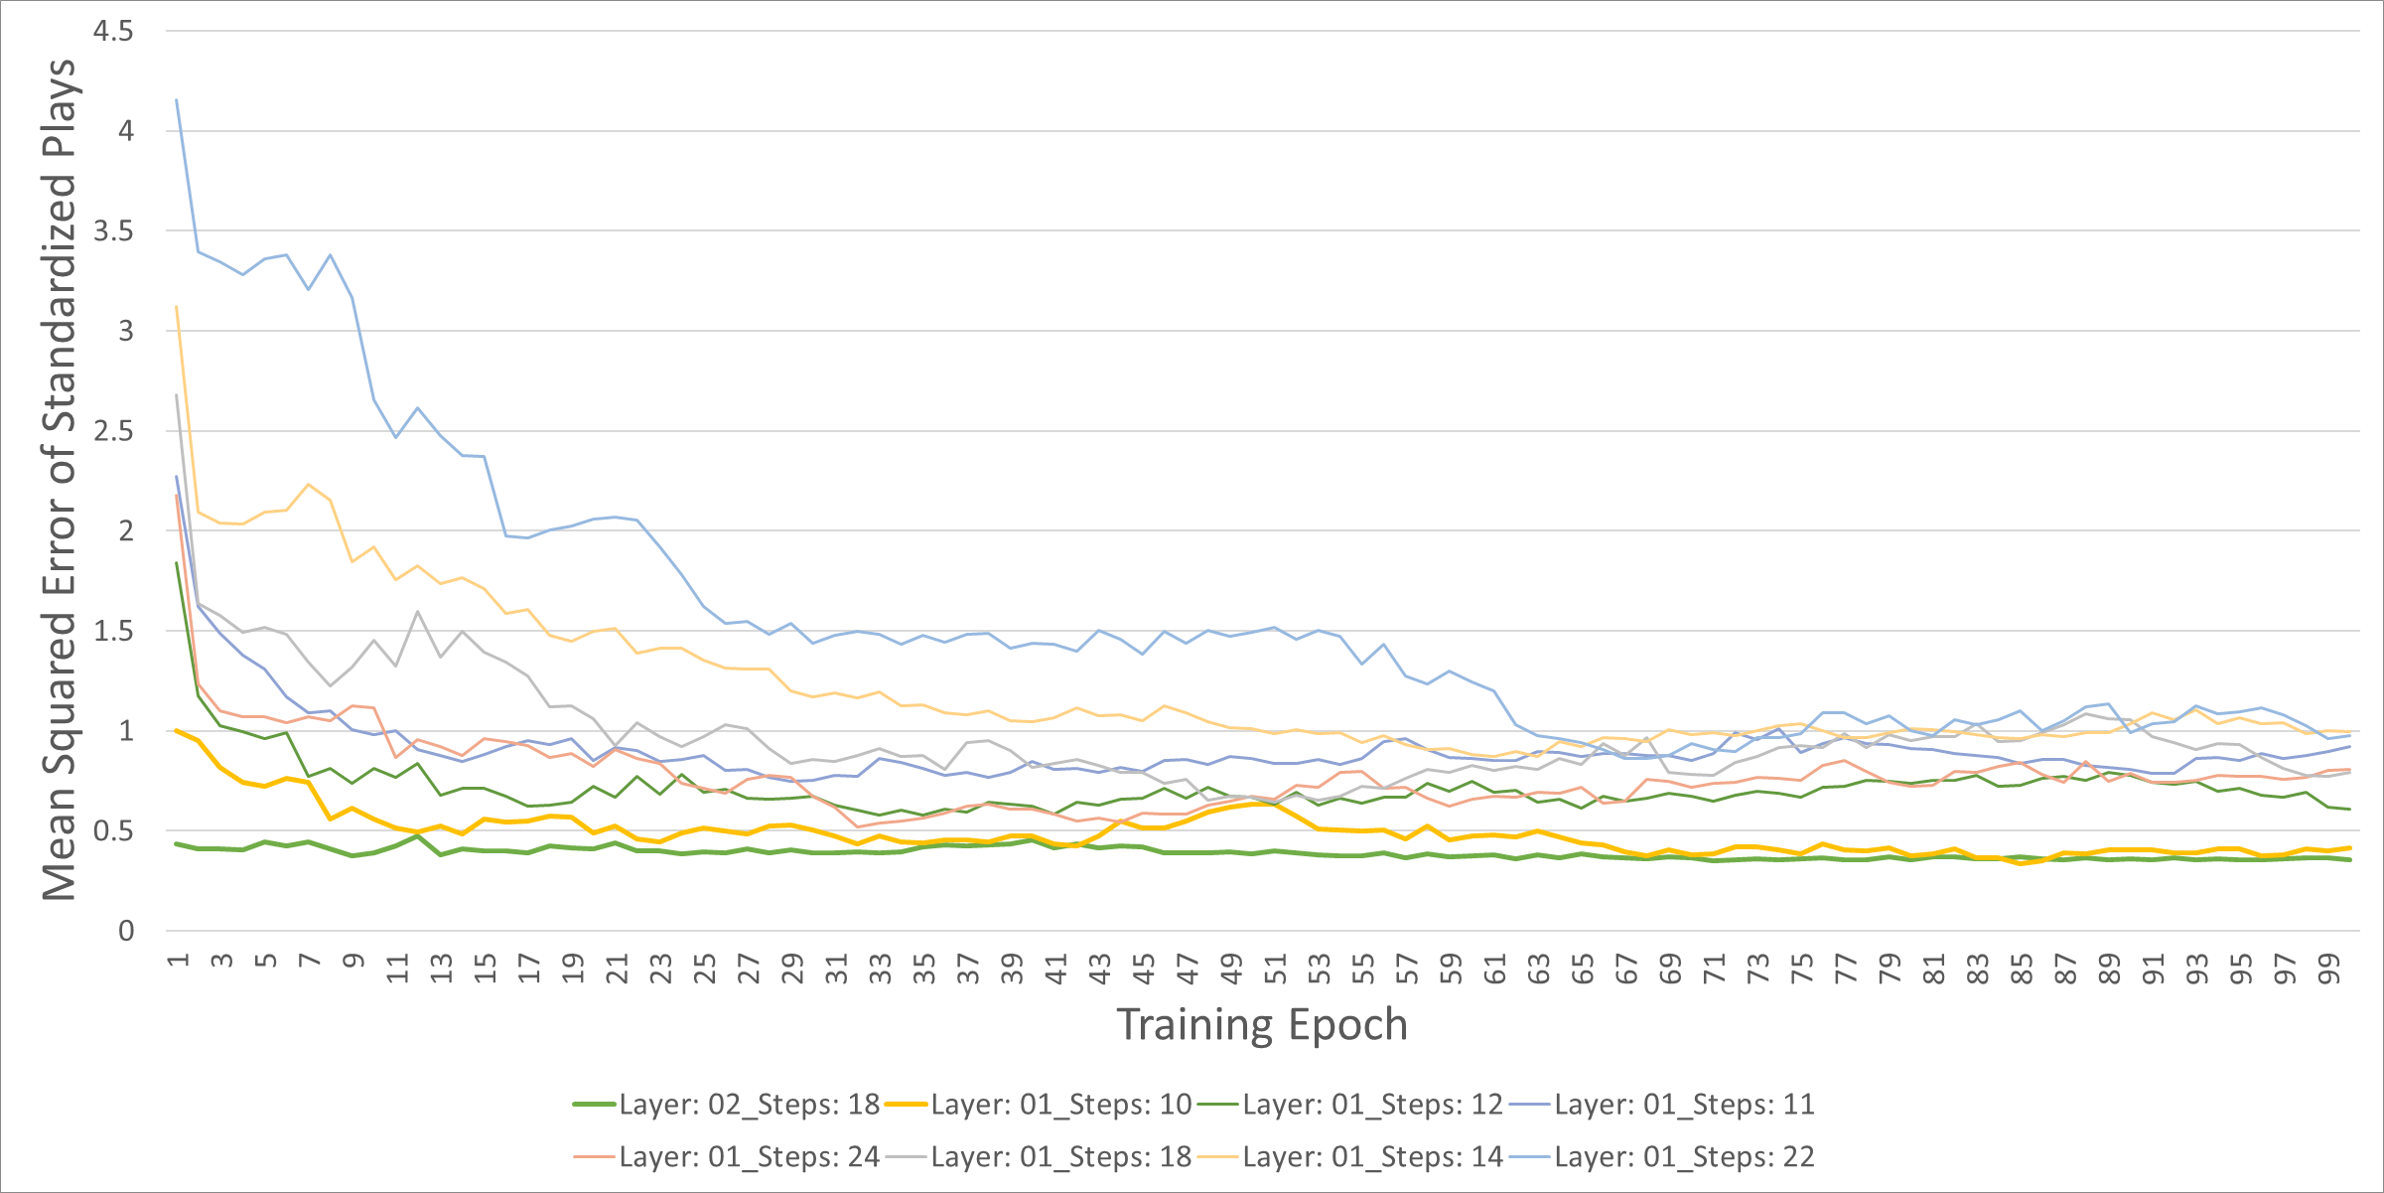
\includegraphics[width=0.45\textwidth]{result_user_3.png}
            \caption{Sample of Model Performance for User 3}
            \label{fig:results-user-3}
        \end{figure}
        
%%%%%%%%%%%%%%%%%%%%%%%%%%%%%%%%%%%%%%%%
%%%%% CRITICISMS
%%%%%%%%%%%%%%%%%%%%%%%%%%%%%%%%%%%%%%%%
    \subsection{Criticisms}
    For all users, there were some model combinations that had diverging loss, most commonly when the number of time steps was low. The researchers assume that this is due to the nature and purpose of LSTM networks, a longer time step (history) creates better performance. After all, the goal is to learn a pattern over time and remember that pattern to make predictions.  However, it is worth noting that this was not true 100\% of the time.  As one can see in figure \ref{fig:results-divergent}, these low time-step models provide poor performance and a divergent mean squared error. Some models even with larger time step values also performed poorly, most likely due to a bad random initialization.
        \begin{figure}
            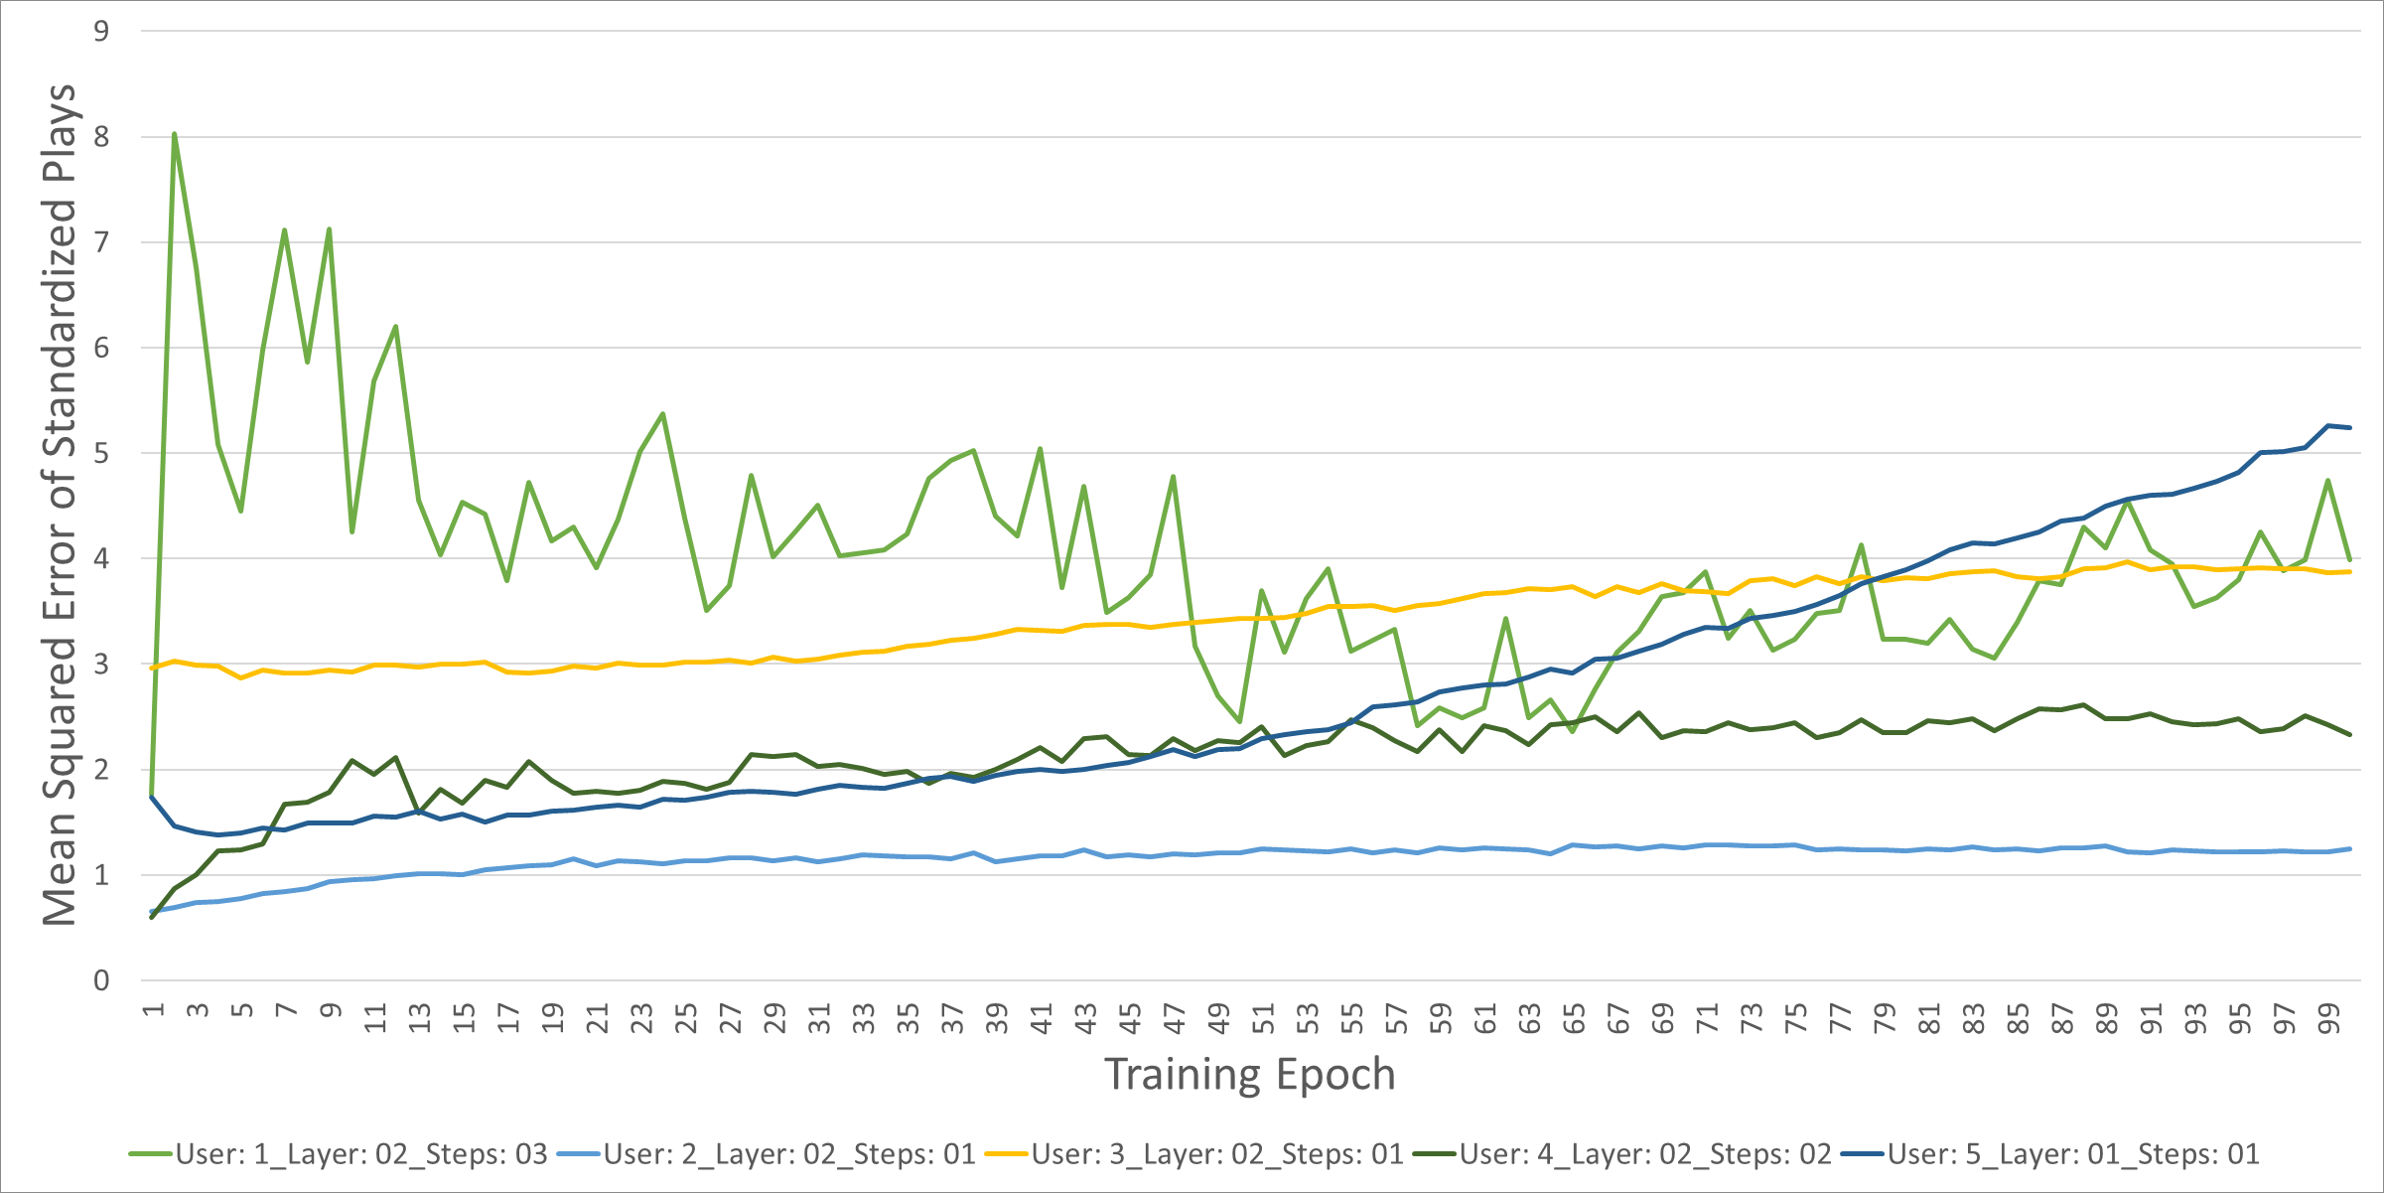
\includegraphics[width=0.45\textwidth]{result_diverging.png}
            \caption{Examples of Divergent Models Due to Too Few Time Steps}
            \label{fig:results-divergent}
        \end{figure}
